% Dépendences : 
% pip install pygments
% Python3

% Installation de pip : (Windows)
% wget https://bootstrap.pypa.io/get-pip.py
% python3 get-pip.py
% Rajout dans le PATH, cf. message

% Compilation : 
% 1 - pdflatex --shell-escape rapport.tex
% 2 - bibtex --shell-escape rapport.aux
% 3 - pdflatex --shell-escape rapport.tex


% Citations de sources bibliographiques
% http://merkel.texture.rocks/Latex/natbib.php?lang=fr

% Documentation classe 
% https://www.elsevier.com/__data/assets/pdf_file/0009/56844/elsdoc2.pdf
\documentclass[3p, twocolumn]{elsarticle}
\usepackage[T1]{fontenc}
\usepackage[utf8]{inputenc}
\usepackage{csquotes}
\usepackage[french]{babel}
\usepackage{fancyhdr}
\usepackage{physics}
\usepackage{titlesec} % titlespacing %
\usepackage{listings} % lstnewenvironment %
\usepackage{textcomp}
\usepackage{regexpatch}
\usepackage[usenames,dvipsnames,svgnames,table]{xcolor}
\usepackage{parskip}
\usepackage{graphicx}
\usepackage{pdfpages}
\usepackage{caption}
\usepackage{titletoc}
\usepackage{mathrsfs}
\usepackage[table]{xcolor}
\usepackage{minted}
\usepackage[french]{algorithm2e}% http://tug.ctan.org/macros/latex/contrib/algorithm2e/doc/algorithm2e.pdf
\usepackage{amsmath,amssymb,amsfonts}
\usepackage{graphicx}
\usepackage{textcomp}
\usepackage{xcolor}
\usepackage[hidelinks]{hyperref}
\usepackage[toc,page]{appendix}
\renewcommand{\appendixtocname}{Annexes}
\renewcommand{\appendixpagename}{Annexes}
\DeclareMathOperator{\Hessian}{H}
\DeclareMathOperator{\Jacobian}{J}
\hypersetup{
  colorlinks = false,
  citecolor=black,
  filecolor=black,
  linkcolor=black,
  urlcolor=black
}
\newtheorem{thm}{Théorème}
\newtheorem{lem}[thm]{Lemme}
\newtheorem{definition}{Définition}[section]
\newdefinition{rmk}{Remarque}[section]
\newdefinition{exemple}{Exemple}[section]
\newproof{pf}{Preuve}[section]

\newcounter{linecounter}
\newcommand{\linenumbering}{\ifthenelse{\value{linecounter}<10}{(0\arabic{linecounter})}{(\arabic{linecounter})}}
\renewcommand{\line}[1]{\refstepcounter{linecounter}\label{#1}\linenumbering}
\newcommand{\resetline}[1]{\setcounter{linecounter}{0}#1}
\renewcommand{\thelinecounter}{\ifnum \value{linecounter} > 9\else 0\fi \arabic{linecounter}}

% Enlever le footer spécifique à Elsevier

\keywordtitle{Mots-clés\,}
\abstracttitle{Résumé}

\makeatletter
\regexpatchcmd*{\@makecaption}{:}{\cA:}{}{}
\regexpatchcmd*{\keyword}{:}{\cA:}{}{}
\def\ps@pprintTitle{%
 \let\@oddhead\@empty
 \let\@evenhead\@empty
 \def\@oddfoot{}%
 \let\@evenfoot\@oddfoot}
% fix english
\xpatchcmd{\printFirstPageNotes}
  {Email addresses}
  {Adresses email}{}{}
\xpatchcmd{\printFirstPageNotes}
  {Email address}
  {Adresse email}{}{}
\regexpatchcmd*{\printFirstPageNotes}{:}{\cA -}{}{}
\makeatother

\begin{document}
\nocite{arxiv:kovalev2019stochastic}
\begin{frontmatter}
    \title{Méthode de Newton et de Quasi-Newton BFGS (Algorithme de BRoyden, Fletcher, Goldfarb et Shanno)}
    \author{Mathilde Rineau}
    \author{Mathilde Le Moel}
    \author{Pascal Quach}
    \author{Félix Poullet-Pagès}

    \begin{abstract}
        La méthode de Newton est une méthode itérative de recherche d'un zéro d'une fonction $g$, qui se repose sur la méthode du point fixe. Elle requiert cependant le calcul coûteux de la dérivée ou matrice jacobienne de $g$ dans le cas d'une fonction à plusieurs variables, et également son inversion. Les méthodes sont qualifiées de quasi-Newton lorsque la matrice jacobienne - généralement son inverse - sont remplacées par une approximation. Appliquée à un problème d'optimisation mono-objectif libre, où l'on cherche l'optimum d'une fonction $f:\mathbb{R}^n\rightarrow \mathbb{R}$, la méthode de Newton force le calcul de la matrice hessienne de $f$, car on cherche les zéros du gradient de $f$. La méthode de Broyden-Fletcher-Goldfarb-Shanno (BFGS) est une méthode quasi-Newton qui se repose sur l'approximation de la matrice hessienne - ou son inverse - par analyse des gradients successifs. La matrice hessienne n'est pas calculée à chaque itération de la méthode, mais mise à jour itérativement en prenant une estimation de la matrice hessienne initiale.
    \end{abstract}
\end{frontmatter}

\cleardoublepage
\tableofcontents

\cleardoublepage
\section{Notations}
\begin{enumerate}
    \item $\Jacobian_{f}(x)$ désigne la matrice jacobienne de la fonction $f$ évaluée en $x$.
    \item $\nabla f(x)$ désigne le gradient de la fonction $f$ évaluée en $x$.
    \item $\Hessian_{f}(x)$ désigne la matrice hessienne de la fonction $f$ évaluée en $x$.
    \item $\nabla^2_{f}(x)$ désigne la dérivée du gradient de la fonction $f$ évaluée en $x$.
\end{enumerate}

\section{Méthode de Newton}
\subsection{Origines}
La méthode de Newton apparaît pour la première fois au XVIIème siècle dans l'ouvrage \emph{De analysi per aequationes numero terminorum infinitas} (1669), puis une seconde fois dans \textit{La méthode des fluxions\footnote{Les fluxions représentent des dérivées}, et les suites infinies}\footnote{Voir \cite{book:newtonfluxions}}, tous deux écrits par Isaac Newton. Elle est à l'époque appliquée au cas particulier des recherches des racines d'un polynôme. Ses travaux ne seront malheureusement publiés que de façon posthume à partir de 1736. Cette méthode est simplifiée par Joseph Raphson dans \textit{Analysis aequationum universalis} (1690), et c'est généralement la version de Raphson qui est utilisée aujourd'hui. Pour ces raisons, on a tendance à parler de la méthode de Newton-Raphson. Les travaux de Thomas Simpson élargissent cette méthode itérative à la recherche de racines d'un plus grande nombre d'équations, notamment les équations non linéaires.
\begin{figure}[htbp]
    \centering
    \includegraphics[width = 0.3\textwidth]{La_méthode_des_fluxions_et_[...]Newton_Isaac_bpt6k62411f_40.jpg}
    \caption{Extrait de l'ouvrage \textit{La méthode
            des fluxions, et les suites infinies} expliquant la méthode de Newton}
    \label{fig:fluxion_newton_method}
\end{figure}

\subsection{Principe}
La méthode de Newton-Raphson est une méthode de recherche des racines de fonctions à valeurs réelles.
\begin{definition}
    Étant donné une fonction $G: \Omega\subset\mathbb{R}^n\longrightarrow \mathbb{R}^m$, $G$ différentiable et une valeur initiale $x_0\in \Omega$ donnée, alors la suite $(x_k)_{k\in \mathbb{N}}$ définie par
    \begin{equation}
        x_{k+1} = x_k - \Jacobian^{-1}_G(x_k)\cdot G(x_k)
        \label{eq:iteration-newton-rn}
    \end{equation}
    converge vers une racine $x_*$ de $G$, à condition que $x_0$ soit suffisamment proche de $x_*$.
\end{definition}
\begin{rmk}
    $\Jacobian_G$ est préférablement inversible. Si la matrice n'est pas carrée, on peut se servir du pseudo-inverse de matrices non-carrés; à gauche s'il y a plus de contraintes que de variables; à droite s'il y a plus de variables que de contraintes. Si la matrice est carrée non inversible, on peut se servir du pseudo-inverse de Moore-Penrose.
    \begin{exemple}
        Trouver les racines de $F
        \begin{pmatrix}
            x\\y
        \end{pmatrix}
        =
        \begin{pmatrix}
            x^2+y^2-1\\
            y+x
        \end{pmatrix}$ est un problème "bien contraint", la matrice jacobienne est inversible. Si l'on décide de rajouter une contrainte, par exemple $y-\frac{\sqrt2}{2}$, alors le jacobien n'est pas carré, on peut se servir du pseudo-inverse pour appliquer la méthode de Newton-Raphson.
    \end{exemple}
\end{rmk}
\begin{rmk}
    Il est important que la fonction $G$ admette un développement de Taylor d'ordre 1 dans un voisinage des racines $x_*$. En effet, l'existence de ce développement justifie en partie la convergence de la méthode itérative. Itérativement, on souhaite contraindre la suite $(x_k)_{k\in \mathbb{N}}$ telle qu'à toute itération $k$, $G(x_{k+1})=0$. On considère le développement de Taylor \textit{d'ordre 1} au voisinage de $x_{k}$.
    \begin{equation*}
        G(x_{k+1})\simeq G(x_k)+\Jacobian_G(x_k)\cdot(x_{k+1}-x_k)
    \end{equation*}
    Dans l'idée, pour s'approcher d'une racine de $G$, on applique la contrainte souhaitée $G(x_{k+1})=0$, et on en déduit l'expression de l'équation \ref{eq:iteration-newton-rn}. L'erreur à chaque itération est dûe à l'approximation par le développement de Taylor : on a négligé son reste.
\end{rmk}
\begin{rmk}
    La méthode de Newton-Raphson peut être appliquée aux fonctions holomorphes, fonctions à valeurs complexes, définie et dérivable en tout point d'un ouvert de $\mathbb{C}$.
\end{rmk}

\subsection{Interprétation géométrique}
Pour mieux comprendre cette méthode itérative, il est plus simple de raisonner en deux dimensions. On considère la fonction $g :\Omega\subset\mathbb R^2 \rightarrow \mathbb R$.

La formule itérative équivalente est la suivante :
\begin{equation}
    x_{k+1}=x_k-\frac{g(x_k)}{g'(x_k)}
    \label{eq:iteration-newton-r2}
\end{equation}
En passant tous les membres à gauche dans l'équation \ref{eq:iteration-newton-r2}, on obtient $g'(x_k)(x_{k+1}-x_k)+g(x_k)=0$. On reconnaît ici l'équation de la tangente à $g$ en $x=x_k$ évaluée au point $(x_{k+1},0)$.
Ce point correspond à l'intersection entre la tangente à $g$ en $x_k$ et la droite des abscisses.

La figure \ref{fig:nr-iterations-1} fournit un exemple visuel des itérations de la méthode de Newton-Raphson en deux dimensions. La fonction $g$ est définie par $g(x)=\frac{1}{12}x^3+\frac18x^2-3x$, et on choisit comme valeur de recherche initiale $x_0=-3.5$. On dessine les tangentes successives, et leurs intersections, jusqu'à s'approcher raisonnablement d'une racine de $g$.

\begin{figure}[htbp]
    \centering
    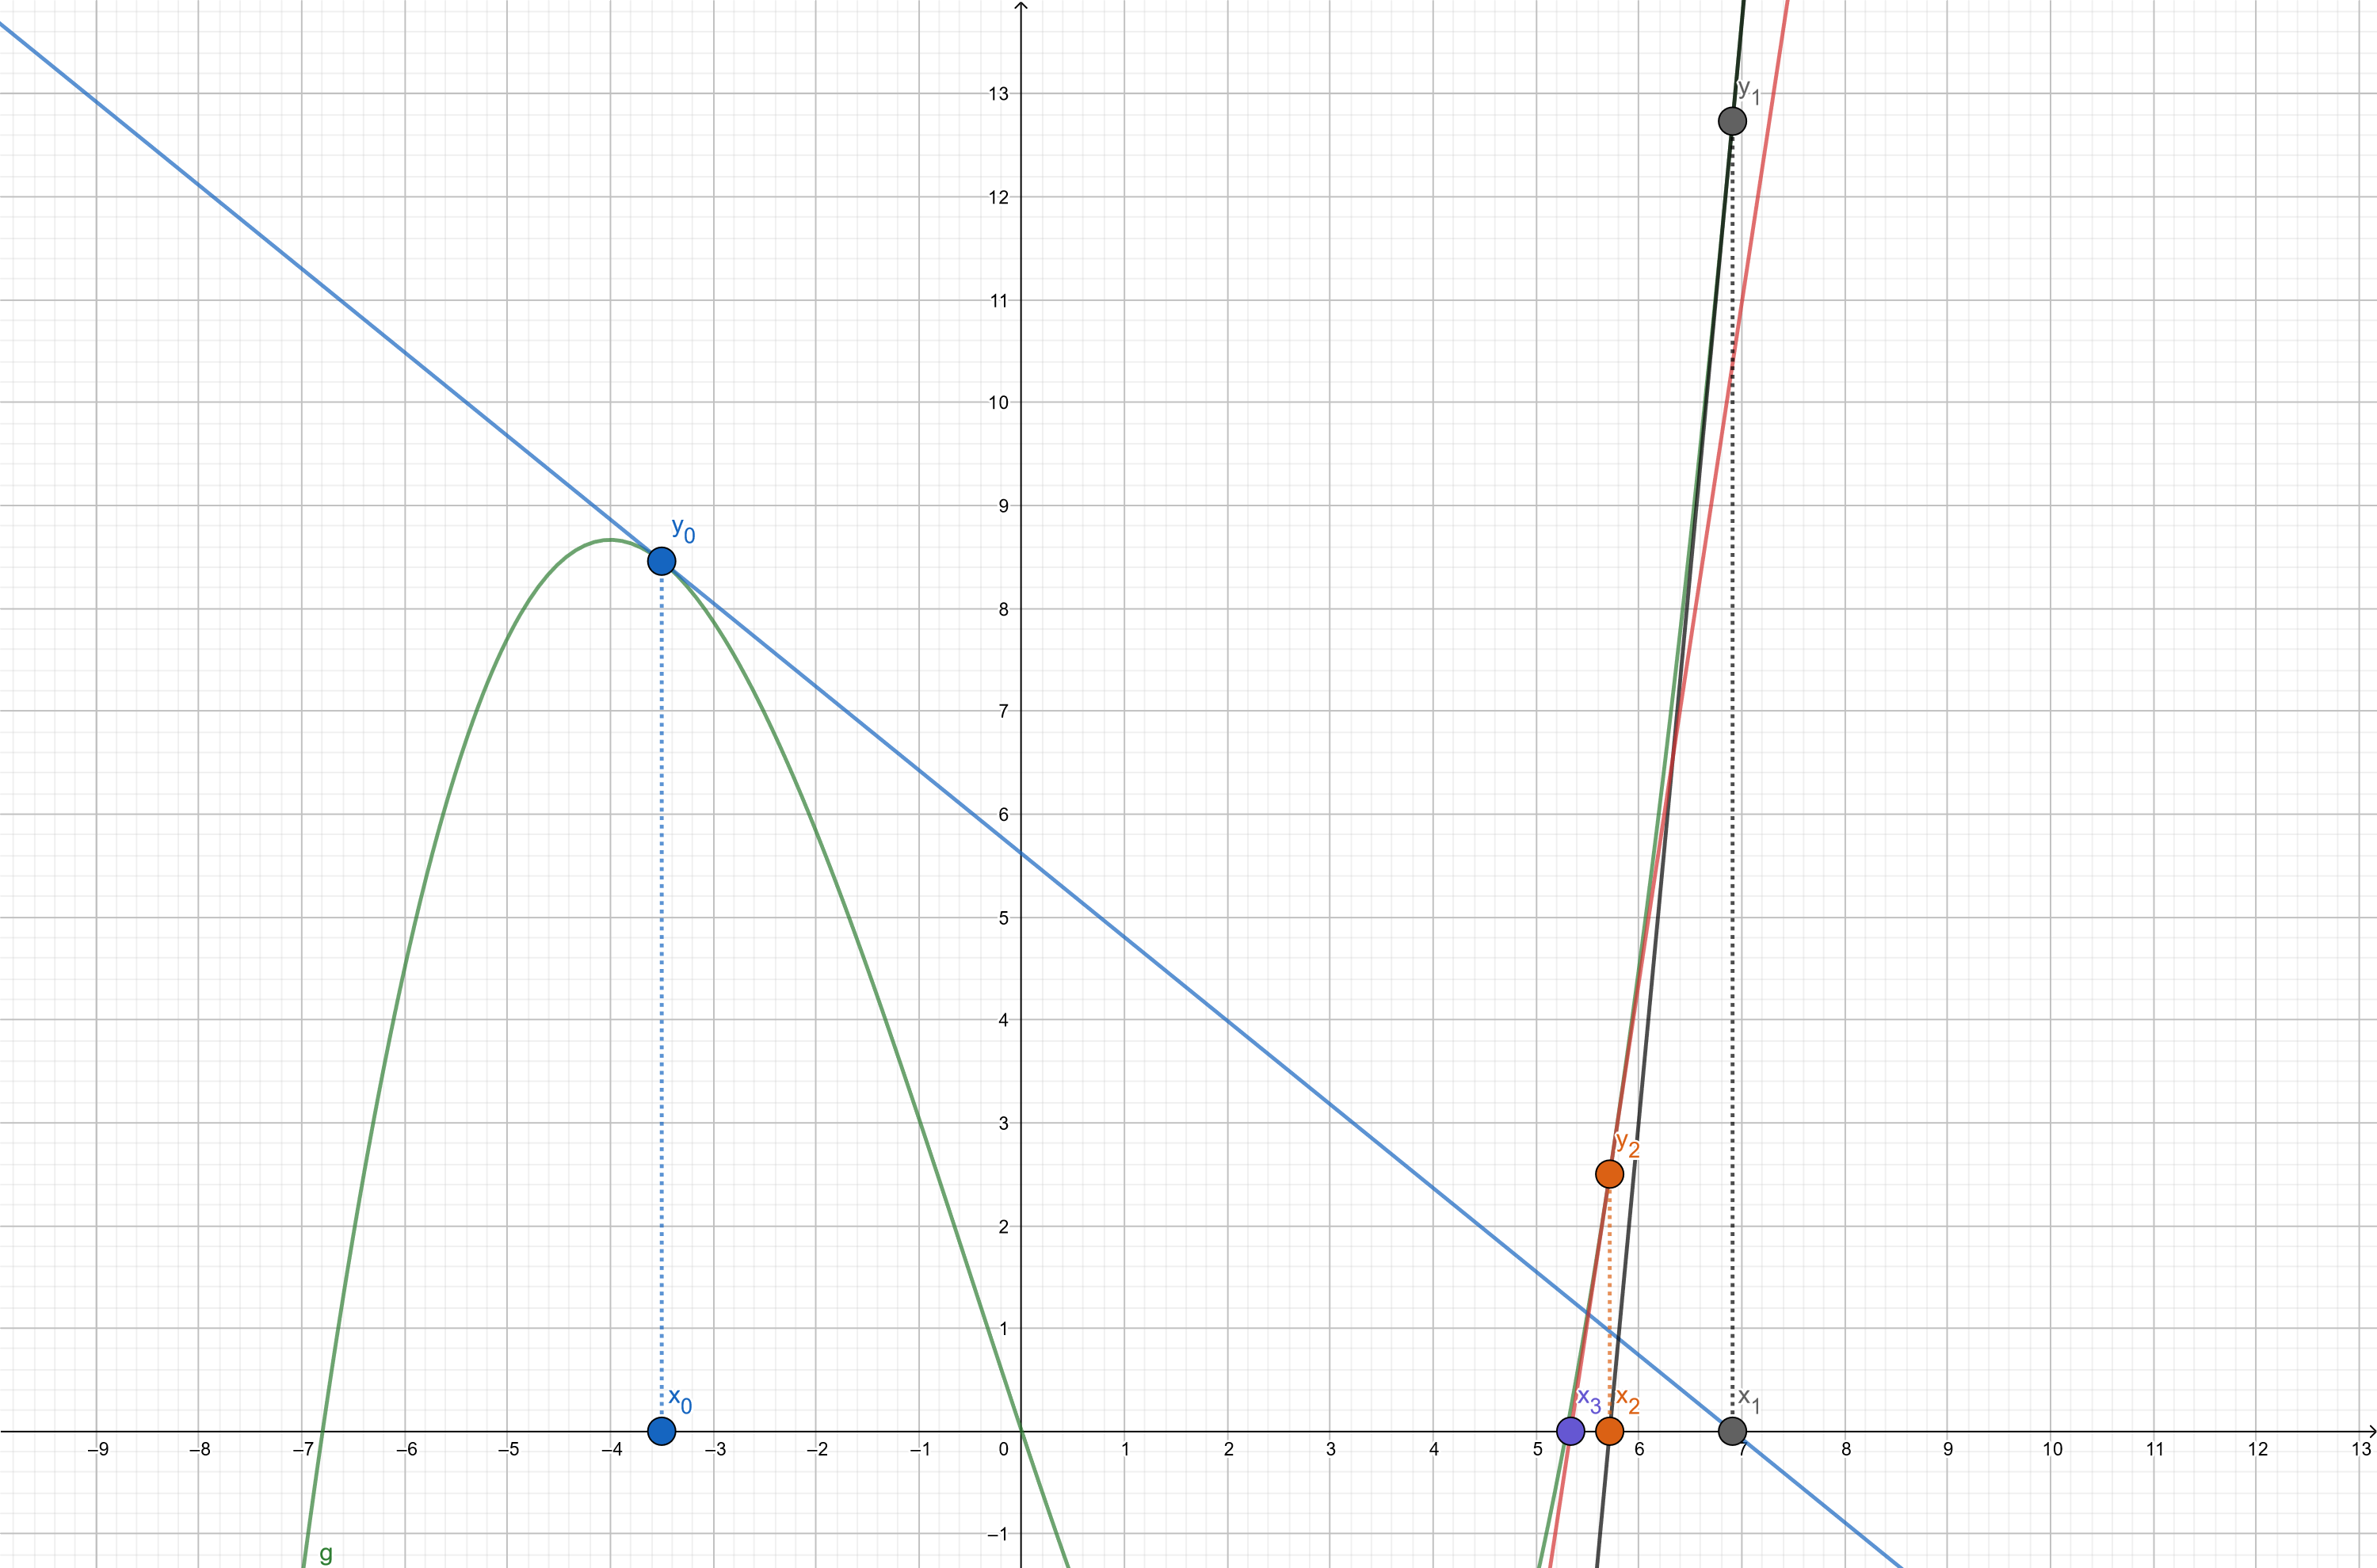
\includegraphics[width = 0.3\textwidth]{iteration-newton-1.png}
    \caption{Itérations de l'algorithme de Newton-Raphson pour la fonction $g$ définie par $g(x)=\frac{1}{12}x^3+\frac18x^2-3x$ telle que $x_0=-3.5$}
    \label{fig:nr-iterations-1}
\end{figure}

\begin{rmk}
    Le choix de la valeur de recherche initiale est important. Si l'on choisit $x_0=-4$, la pente de la tangente de $g$ en $x_0$ est nulle, et les itérations suivantes ne sont pas définies car la dérivée est nulle : la méthode itérative s'arrête. Ce choix a tout autant d'importance en dimensions supérieures à 2.
\end{rmk}


\subsection{Qualités et faiblesses}
\subsubsection{Vitesse de convergence}
La convergence est d'ordre quadratique au voisinage d'une solution. Si la suite converge, alors :

\begin{equation*}
    \lVert x_{k+1}-x^{*}\rVert \leq \gamma\lVert x_{k}- x^{*}\rVert^{2}, \gamma >0
    \label{eq:convergence-nr}
\end{equation*}

La méthode de Newton-Raphson converge quadratiquement au voisinage d'une solution, ce qui est remarquable. Malheureusement, cet ordre de convergence n'est valable que localement, ce qui limite son intérêt. De plus, il est généralement difficile d'expliciter "le voisinage de $x_*$".

\subsubsection{Cas de non convergence}
Dans certains cas, la méthode de Newton-Raphson ne converge pas.

 \textbf{Domaine de définition} - Le calcul de $x_{k+1}$ peut mener à une valeur en dehors du domaine de définition $\Omega$ de $G$.

 \textbf{Différentiabilité} - Si le gradient de la fonction $G$, $\Jacobian_G(x)$ a un comportement anormal, e.g. il n'est pas définie au voisinage d'une racine $x_*$, c'est-à-dire que $G$ n'est pas différentiable en $x_*$, alors la méthode ne peut pas converger.

 \textbf{Optima locaux} - Au cours des itérations de la méthode, l'algorithme peut éventuellement s'arrêter sur un optimum. La méthode oscille (ou s'arrête si on doit diviser par 0), car la matrice jacobienne sera nul. La matrice jacobienne peut être nulle, dans ce cas-là la méthode est "bloquée" : $x_{k+1} = x_k$. Ce cas de non-convergence correspond en deux dimensions à la pente nulle de la tangente en $x_k$.

\textbf{Valeur initiale} - Toutefois, la non-convergence de la méthode de Newton-Raphson est le plus souvent due au mauvais choix de la valeur initiale $x_{0}$. Il est important d'itérer à partir d'une estimation raisonnable de la solution voulue.

\textbf{Convergence} - En somme, pour une fonction quelconque, il n'existe aucune garantie que la méthode de Newton-Raphson converge. Il faudra s'assurer que la fonction ait certaines propriétés particulières - notamment sa stricte convexité - pour appliquer la méthode de Newton-Raphson à un problème d'optimisation. 

\begin{exemple}
    On considère la fonction $G:\mathbb R^n\rightarrow \mathbb R^n$ définie par $G(x)=\left(\lvert x_i\rvert^{\frac12}\right)_{1\leq i\leq n}$. La méthode itérative de Newton-Raphson mène à $x_{k+1}=-x_k$. \footnote{Les détails du calcul sont précisés dans l'annexe \ref{ap:calcul-exemple-nr}.}
    \label{ex:newton-raphson-non-differentiable}
    La méthode Newton-Raphson ne converge pas, et on oscille entre deux points. Effectivement, comme $G$ n'est pas différentiable en $x_k=\overrightarrow 0$, la matrice jacobienne n'y est pas définie. Pour toute valeur $x_0\neq \overrightarrow 0$, l'algorithme ne convergera pas. En figure \ref{fig:nr-iterations-2}, les itérations pour la fonction $G$ lorsque $n=1$.
    \begin{figure}[htbp]
        \centering
        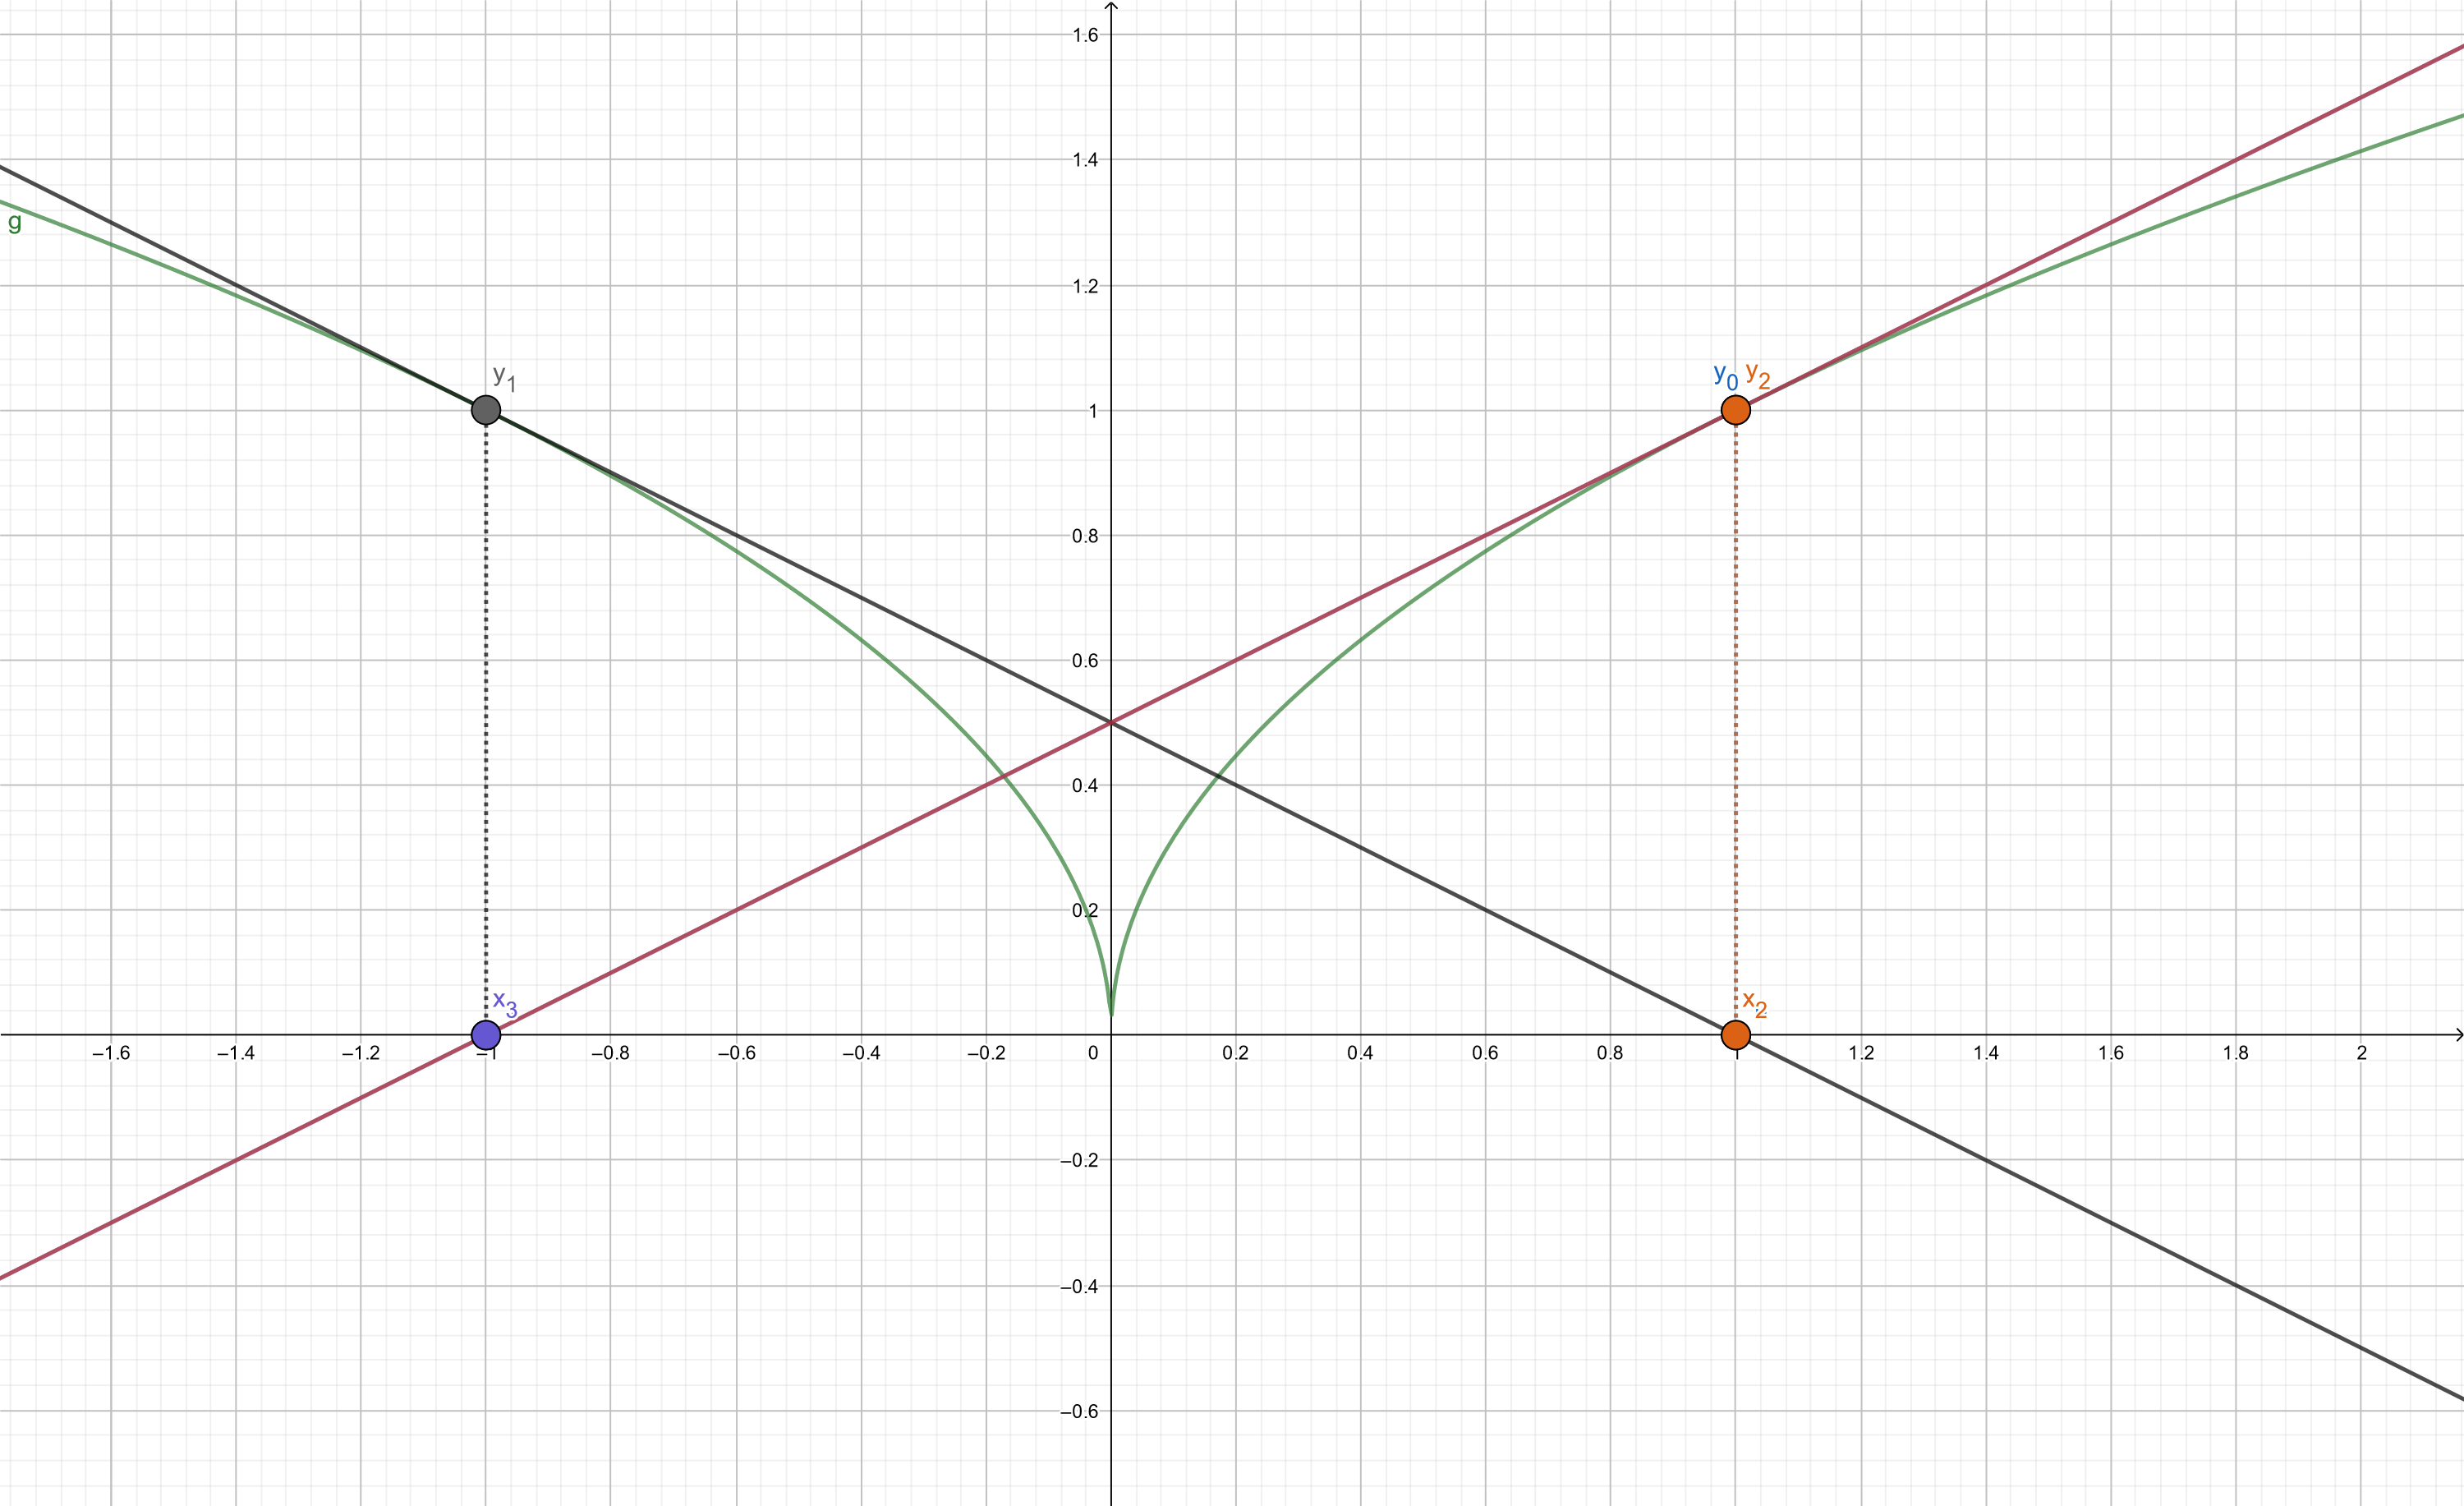
\includegraphics[width = 0.3\textwidth]{iteration-newton-2.png}
        \caption{Itérations de la méthode de Newton-Raphson pour $g(x) = \lvert x \rvert ^{\frac12}$ telle que $x_0 = 1$}
        \label{fig:nr-iterations-2}
    \end{figure}
\end{exemple}

\subsubsection{Cas de convergence lente $f:\mathbb{R}\rightarrow \mathbb{R}$}
Lorsqu'une racine est au moins de multiplicité 2, alors la convergence n'est plus d'ordre quadratique mais presque linéaire. Cependant, si cette multiplicité est connue, il est possible de modifier la méthode pour retrouver une convergence quadratique locale. En notant $m$ cette mutiplicité, on obtient :
% TODO : Jacobien ? 
\begin{equation*}
    x_{n+1}=x_{n}-m\frac{f(x_{n})}{f'(x_{n})}    
\end{equation*}

\begin{rmk}
S'il existe deux racines, proches l'une de l'autre, l'algorithme aura besoin de plusieurs itérations pour s'approcher de l'une d'entre elles.
\end{rmk}

\subsubsection{Coût de la méthode}
Le coût de calcul de la méthode de Newton est important. En effet, à chaque itération, il est nécessaire d’évaluer la jacobienne de $f$. Or, cette évaluation est relativement coûteuse.

\subsection{Application à un problème d'optimisation mono-objectif libre}
La recherche de l'optimum d'une fonction s'apparente à la recherche des zéros de son gradient.
Soit le problème d'optimisation, avec $f:\Omega \subset \mathbb{R}^n \rightarrow \mathbb{R}$
\begin{equation}
    (\mathscr{P}):\quad\min_{x\in \Omega} f(x)
    \label{eq:probleme-opt}
\end{equation}
La méthode de Newton-Raphson peut donc être appliquée au problème d'optimisation (\ref{eq:probleme-opt}) en choisissant $g(x)=\nabla f(x)$.
\begin{definition}
    Soit une fonction $f:\Omega \in \mathbb{R}^n\rightarrow \mathbb{R}$, deux fois dérivable, strictement convexe et de hessienne K-lipschitzienne dans un voisinage de $x_*$. Soit une valeur initiale $x_0\in Omega$, alors la suite $(x_k)_{k\in \mathbb{N}}$ définie par
    \begin{equation}
        x_{k+1}=x_k-\nabla^{2}f(x_k)^{-1}\cdot \nabla f(x_k)
        \label{eq:nr-opt-mono}
    \end{equation}
    converge quadratiquement vers $x_*$, le minimum de $f$, dans son voisinage.
\end{definition}

\subsubsection{Convergence restreinte au voisinage de $x_*$}
Encore une fois, l'intérêt de la méthode de Newton-Raphson est limitée par la restriction sur la valeur initiale $x_0$ qui doit être dans un voisinage de $x_*$.
Ce problème peut être résolu en ajoutant une phase de recherche linéaire dans la direction
\begin{equation*}
    d_{k} = -\nabla ^{2}f(x_{k})^{-1} \nabla f(x_{k})
\end{equation*}
telle que la suite $(x_k)_{k\in \mathbb{N}}$ soit définie par
\begin{equation}
    x_{k+1}=x_k+t_k\cdot d_k
    \label{eq:nr-opt-mono}
\end{equation} 
avec $t_k$ le pas résultant d'une recherche linéaire.
Compte tenu des propriétés choisies pour $f$, $d_k$ est une direction de descente en $x_k$. En effet, la stricte convexité de $f$ implique que la hessienne soit strictement définie positive.
\begin{rmk}
    Si la stricte convexité de $f$ n'est pas vérifiée, il faudra vérifier que la hessienne est strictement définie positive. Ce résultat n'est pas garanti. S'il existe une solution au problème, on sait tout au plus que $\nabla^2f(x_*)>0$.
\end{rmk}

\subsubsection{Optima locaux}
Cependant, la convergence de la méthode de Newton-Raphson n'implique pas l'obtention d'un minimum global de $f$, particulièrement si la valeur initiale $x_0$ est mal choisie. La fonction peut posséder plusieurs minima. Pour pallier à ce problème, différents solutions existent. Parmi elles, des méthodes hybrides (utilisation d'un algorithme génétique en parallèle de la méthode) ont été développé.

La méthode \textit{Hybrid Genetic Deflated Newton} (HGBN) \cite{art:Noack_Funke_2017} est particulièrement équipée pour optimiser des fonctions qui possède de nombreux optima locaux. Elle consiste en l'application locale de multiples algorithmes de Newton-Raphson sur une population d'individus - les valeurs initiales - pour identifier des optima et les rendre introuvable ($deflation$). La nouvelle génération est sélectionnée par survie du plus adapté, et on recherche de nouveau les optima jusqu'à les avoir tous trouvé.

HGBN converge vers un optimum global, et réduit significativement le nombre d'évaluations de fonctions nécessaire. 

\begin{rmk}
    Concernant la recherche d'un optimum global, une alternative raisonnable serait la méthode du recuit simulé (\textit{simulated annealing} en anglais). Sur des problèmes où l'optimum global est enfoui parmi de multiples optima locaux, le recours à cette méthode est un choix raisonnable, quitte à être contraint à paramétrer l'algorithme manuellement, étant donné que c'est une méthode métaheuristique.
\end{rmk}

\subsubsection{Nombre d'évaluations, de calcul}
Les itérations de la méthode de Newton-Raphson nécessite l'évaluation du gradient, et de l'inverse de la hessienne de $f$ (matrice de taille $n\times n$). Dépendant de l'implémentation de l'algorithme, l'inversion de la hessienne de $f$ est également à prendre en compte, e.g. si on décide de ne pas l'inverser manuellement. La méthode de Newton-Raphson est donc informatiquement coûteuse, l'inversion d'une matrice étant souvent implémentée par la résolution d'un système d'équations linéaires.

\subsubsection{Propriétés de $f$}
La méthode de Newton-Raphson est valable si certaines propriétés de $f$ sont vérifiées : stricte convexité, deux fois différentiable. Cela restreint considérablement le champ d'application de la méthode de Newton-Raphson.

Si la fonction $f$ est seulement convexe, la hessienne de $f$ est semi-définie positive. Elle n'est donc pas forcément inversible. 

\subsubsection{Vers les méthodes de quasi-Newton}
La nécessité que $f$ soit deux fois différentiable, et strictement convexe, ainsi que le coût relativement élevé de calcul des itérations de la méthode de Newton-Raphson est une faiblesse majeure de l'algorithme.

Cependant, il est possible d'approximer la hessienne (ou son inverse) pour réduire à la fois les restrictions placées sur $f$, et réduire les coûts de calcul. 

\section{Méthode de BFGS}
% Broyden
% méthodes à métrique variable
% méthodes sécante générale
% méthode quasi-Newton
% Méthode Broyden : parenthèse rapide
% DFP : correction rang 2, conserve B > 0
% BFGS : principe (update sur les gradients), modèle quadratique (Taylor), relation quasi-Newton, équation sécante, propriétés (B > 0, forall k, directions conjuguées), recherche linéaire (WolfePoweel ou Goldstein) + remarque V.2.4.
% Remarques : Famille Broyden, Dualité, Remarques sur l'estimation de l'inverse. (pas toujours le cas), L-BFGS
% 
\subsection{Origines}
La méthode de Davidon (1959)\cite{art:Davidon_1991} qu'il nomme lui-même méthode à métrique variable est la base de nombreux travaux. Cette méthode de résolution de problèmes d'optimisation non-linéaire libre a la particularité de considérer une matrice variable d'une itération à une autre, i.e. la matrice $B$ estimation de l'inverse de la hessienne. Parmi les mathématiciens s'étant penché sur ces travaux, Fletcher et Powell proposent en 1963 une variation de la méthode à métrique variable (DFP), dont Broyden louera les nombreuses qualités en 1970, en la comparant à ses travaux précédent de 1967. Il s'avance même en qualifiant la méthode DFP de meilleur algorithme pour résoudre un problème d'optimisation libre, où l'expression explicite du gradient est accessible. En 1967, Broyden décrit la classe d'algorithmes qu'il nomme les méthodes de Quasi-Newton, généralisation de la méthode de la sécante dans le cas multidimensionnel basée sur les travaux de Wolfe (1659) et de Barnes (1965).

La méthode de Broyden-Fletcher-Goldfarb-Shano (BFGS) ...
\subsection{Principe}
\subsection{Résultats connus}
\subsection{Qualités et faiblesses}
\section{Implémentation sur SCILAB}
\subsection{Recherche linéaire : condition de Wolfe}
\subsubsection{Algorithme}
\subsubsection{Programme}
\subsubsection{Conditions d'arrêts et précision}
\subsubsection{Difficultées techniques}
\subsection{Méthode de Newton-Raphson}
\subsubsection{Algorithme}
\begin{algorithm}[ht]
    \centering{
        \fbox{
            \begin{minipage}[t]{150mm}
                \footnotesize
                \renewcommand{\baselinestretch}{2.5}
                \resetline
                \begin{tabbing}
                    aaaA\=aaaA\=aaA\=aaA\=aaA\=aaA\kill

                    {\bf  Initialisation :}\\
                    \line{NR-01} \> $g$ := la fonction dont on cherche les racines\\
                    \line{NR-02} \> $\nabla g$ := l'expression analytique du gradient de $g$\\
                    \line{NR-03} \> $k = 0$ := le nombre d'itérations actuels\\
                    \line{NR-04} \> $x_0 \in \Omega$ := la valeur initiale de recherche\\
                    \line{NR-05} \> $t_k \in \Omega$ := le pas de l'itération $k$,\\
                    déterminé par une méthode de recherche linéaire\\
                    \line{NR-06} \> $\varepsilon \in \mathbb{R}^+_*$ := la marge d'erreur acceptable,\\ le critère d'arrêt\\
                    \line{NR-07} \> $N\in \mathbb{N}$ := le nombre d'itérations maximales\\
                    {\bf Itérations :}\\
                    \line{NR-08} \> {\bf Tant que} $g(x_k) > \varepsilon$ {\bf ET} $k < N$ {\bf faire :}\\
                    \line{NR-09} \>\> $x_{k+1} = x_k - t_k\nabla f^{2}(x_k)^{-2}\cdot \nabla f(x_k)$\\
                    \line{NR-10} \>\> $N = N+1$\\
                    \line{NR-11} \>\> $k = k+1$\\
                    %------------------
                \end{tabbing}
                \normalsize
            \end{minipage}
        }
        \medbreak
        \caption{Algorithme de la méthode de Newton-Raphson}
        \label{algo:newton_raphson}
    }
\end{algorithm}
\subsubsection{Programme}
\subsubsection{Conditions d'arrêts et précision}
\subsubsection{Difficultées techniques}
\subsection{Méthode de BFGS}
\subsubsection{Algorithme}
\subsubsection{Programme}
\subsubsection{Conditions d'arrêts et précision}
\subsubsection{Difficultées techniques}
\subsection{Affichage des résultats}
\subsubsection{Indicateurs possibles}
\subsection{Exemples d'optimisation}
\subsubsection{Méthode de Newton}
% \paragraph{Exemple convergent}
% \paragraph{Exemple divergent}
% \paragraph{Exemple de convergence difficile}
\subsubsection{Méthode de BFGS}
% \paragraph{Exemple convergent}
% \paragraph{Exemple divergent}
% \paragraph{Exemple de convergence difficile}
\subsection{Critiques et alternatives}
\subsubsection{Critiques}
% \paragraph{Prise en main du langage}
% \paragraph{Temps de calcul}
\subsubsection{Alternatives}

L'utilisation de SCILAB pour implémenter des algorithmes d'optimisation manuellement a été limitée à l'utilisation des outils standard. Une alternative à l'utilisation de l'expression analytique de la dérivée est la différentiation automatique. Sur des fonctions complexes dont l'expression analytique est difficile à calculer, les résultats obtenus sont possiblements convaincants. L'optimisation de programmes utilisant ces techniques est cependant complexe, car elle nécessite une compréhension poussée de la différentiation automatique, notamment de la construction du graphe de calcul. SCILAB possède quelques librairies de différentiation automatique (sciad, diffcode). Eventuellement, l'implémentation des algorithmes aurait pu se détacher de l'interpréteur de SCILAB, et préférer compiler le code en C (en utilisant une librairie de conversion Scilab2C par exemple) en espérant que le code compilé ait une meilleure performance d'exécution que le code interprété. 

Concernant les logiciels d'analyse numérique, la première alternative qui surgit à l'esprit est MATLAB. L'interpréteur de MATLAB est sans équivoque supérieur à celui de SCILAB, moyennant son aspect propriétaire et commercial. 

Egalement, on peut reprocher à SCILAB et MATLAB de restreindre les utilisateurs à un langage de programmation spécifique. Le concurrent populaire sur ce point est l'utilisation du Python, notamment les librairies SciPy et NumPy qui offrent un panel très complet d'outils. La popularité du Python est due en grande partie à la facilité d'apprendre le langage. La présence d'une communauté active et impliquée est aussi l'un de ses points forts. La présence dominante de framework/librairies (PyTorch, NumPy, CuPy, ...) en Python en fait l'un des langages de programmations majeurs.
\begin{enumerate}
    \item 
\end{enumerate}
\section{Applications}
\subsection{Problème 1 : ...}
% \paragraph{Indicateur 1 : courbe de convergence (exemple)}
\cleardoublepage
\begin{appendices}
    \section{Détails de calcul de l'exemple \ref{ex:newton-raphson-non-differentiable}}
    \label{ap:calcul-exemple-nr}
    On considère la fonction $G:\mathbb R^n\rightarrow \mathbb R^n$ définie par $G(x)=\left(\lvert x_i\rvert^{\frac12}\right)_{1\leq i\leq n}$.
    \begin{align*}
        \frac{\partial}{\partial x_i}\lvert x_i\rvert^{\frac12} & = \frac{\partial}{\partial x_i}\left(\sqrt{x_i^2}\right)^{\frac12}                                          \\
                                                                & = \frac12\left(\sqrt{x_i^2}\right)^{-\frac12}\cdot\frac{\partial}{\partial x_i}\left(x_i^2\right)^{\frac12} \\
                                                                & = \frac1{2(\lvert x_i\rvert)^{\frac12}}\frac12\cdot2x_i(x_i^2)^{-\frac12}                                   \\
                                                                & = \frac{x_i}{2\lvert x_i\rvert^{\frac32}}                                                                   \\
        \Jacobian_G(x)                                          & = \begin{cases}
            \frac{x_i}{2\lvert x_i\rvert^{\frac32}} & i=j             \\
            0                                       & \textrm{ sinon}
        \end{cases}
    \end{align*}
    $\Jacobian_G$ est une matrice diagonale, son inverse est simplement $\Jacobian^{-1}_G(x)=\begin{cases}\frac{2\lvert x_i\rvert^{\frac32}}{x_i}&i=j\\0&\textrm{ sinon}\end{cases}$

    \begin{align*}
        x_{k+1} & = x_k - \left(\frac{(x_k)_i}{2\lvert (x_k)_i\rvert^{\frac32}}\right)_{1\leq i\leq n}\cdot \lvert (x_k)_i\vert ^{\frac12} \\
                & = x_k - \left(\frac{2\lvert (x_k)_i \rvert^{2}}{(x_k)_i}\right)_{1\leq i\leq n}                                          \\
                & = x_k - 2x_k                                                                                                             \\
        x_{k+1} & = - x_k
    \end{align*}
\end{appendices}

% Bibliographie
% http://merkel.texture.rocks/Latex/natbib.php?lang=f
\cleardoublepage
\nocite{*}
\biboptions{numbers}
\bibliographystyle{elsarticle-num}
\bibliography{bibliographie}
\phantomsection
\addcontentsline{toc}{section}{Références}

\end{document}
